\documentclass[10pt]{article}
\usepackage{float}
\RequirePackage{eso-pic}
\usepackage{caption}
\captionsetup[table]{labelformat=empty}



\usepackage{geometry}
\geometry{
a4paper,
left=11mm,
right=14mm,
top=37mm,
bottom=14mm,
}



\usepackage{colortbl}
\usepackage{fontspec}
\setmainfont[Ligatures=TeX]{Calibri}



\newcommand\BackgroundPic{%
\put(0,0){%
\parbox[b][\paperheight]{\paperwidth}{%
\vfill
\centering
\includegraphics{MBIE_generic_background.pdf}%
\vfill
}}}



\begin{document}
\thispagestyle{empty}
\AddToShipoutPicture{\BackgroundPic}
\section*{Key Export Statistics\footnotemark - Shelled Beans\footnotemark }
\today\\
\begin{table}[ht]
\centering
{\scriptsize
\begin{tabular}[t]{p{1.8cm}>{\hfill}p{1.4cm}>{\hfill}p{1.4cm}>{\hfill}p{1.6cm}>{\hfill}p{1.9cm}>{\hfill}p{2cm}>{\hfill}p{1.9cm}>{\hfill}p{1.5cm}}
 \textbf{Country} & \textbf{Yearly Qty} & \textbf{Yearly Value} & \textbf{Yearly Price} & \textbf{3Year CAGR(Qty)} & \textbf{3Year CAGR(Value)} & \textbf{3Year CAGR(Price)} & \textbf{Price Elasticity} \\
\hline
Australia & 22,102 & 32.2 & \$1.5 & 4.5\% & 1.3\% & -3\% & -1.5 \\  
Singapore & 343 & 0.5 & \$1.6 & 2\% & 0.3\% & -1.7\% & -1.2 \\  
Fiji & 184 & 0.3 & \$1.6 & 14\% & 14.1\% & 0.1\% & 114.3 \\  
P.N.G & 153 & 0.3 & \$1.7 & 53.4\% & 47.1\% & -4.1\% & -13.0 \\  
Malaysia & 126 & 0.2 & \$1.5 & -0.3\% & -1.8\% & -1.5\% & 0.2 \\  
Indonesia & 73 & 0.1 & \$1.5 & -6.4\% & -8.4\% & -2.2\% & 2.9 \\  
Other & 158 & 0.4 & \$2.3 & 13.3\% & 11.3\% & -1.7\% & -7.8 \\  
Total & 23,138 & 34.0 & \$1.5 & 4.7\% & 1.6\% & -2.9\% & -1.6 \\  
\hline
\end{tabular}
}
\caption{\scriptsize Top 6 Shelled Beans Markets for year ending November - 2015: Quantity('000 kg) Value(NZ\$Mill), Price and their last 3-Year Growth Rates}
\end{table}


\vspace{-0.7cm}



   \begin{figure}[H]
   \centering
    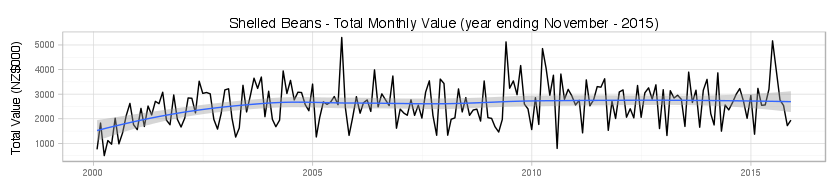
\includegraphics[scale=0.5]{../graphs/monthly_value/shelled_beans_monthly_value.png} \
    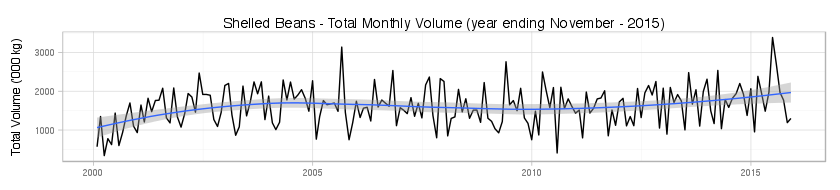
\includegraphics[scale=0.5]{../graphs/monthly_volume/shelled_beans_monthly_volume.png} \
    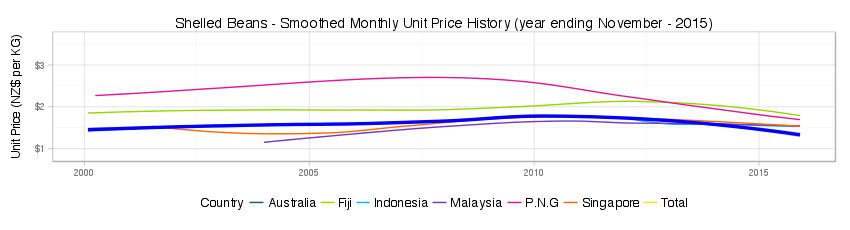
\includegraphics[scale=0.5]{../graphs/smoothed_price/shelled_beans_smoothed_price.png} \
    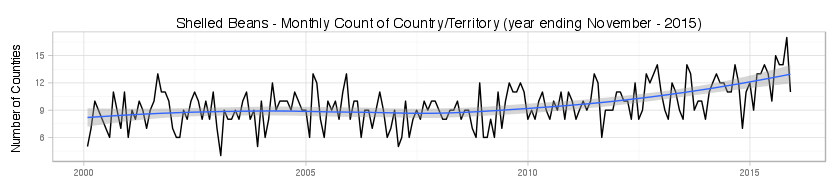
\includegraphics[scale=0.5]{../graphs/monthly_number_countries/shelled_beans_monthly_count.png} \
    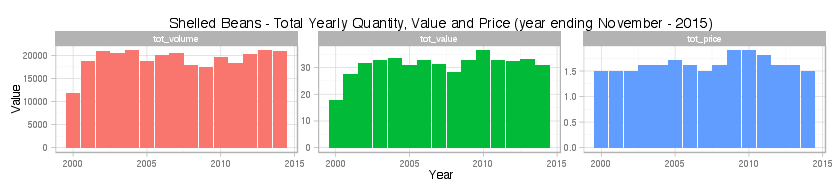
\includegraphics[scale=0.5]{../graphs/yearly_summary/shelled_beans_yearly_summary.png} \
   \end{figure}



\footnotetext[1]{Source: Statistics New Zealand - Overseas Merchandise Trade}
\footnotetext[2]{Harmonised System Codes for Shelled Beans starting with: 200551.}
\end{document}
